%% ============================================================================
%% §4.2.1 Top-Level NPU and Memory Hierarchy  (was: ASIC Frontend)
%% Unified hybrid NPU description.
%% ============================================================================
\subsubsection{Top-Level NPU and Memory Hierarchy}
\label{sec:hw:frontend:top}

Figure~\ref{fig:npu_top} shows the top-level NPU. Three operator engines sit behind a shared Switcher that arbitrates access to the global memories and routes the layer-config descriptor into the active engine.

\begin{figure}[H]
  \centering
  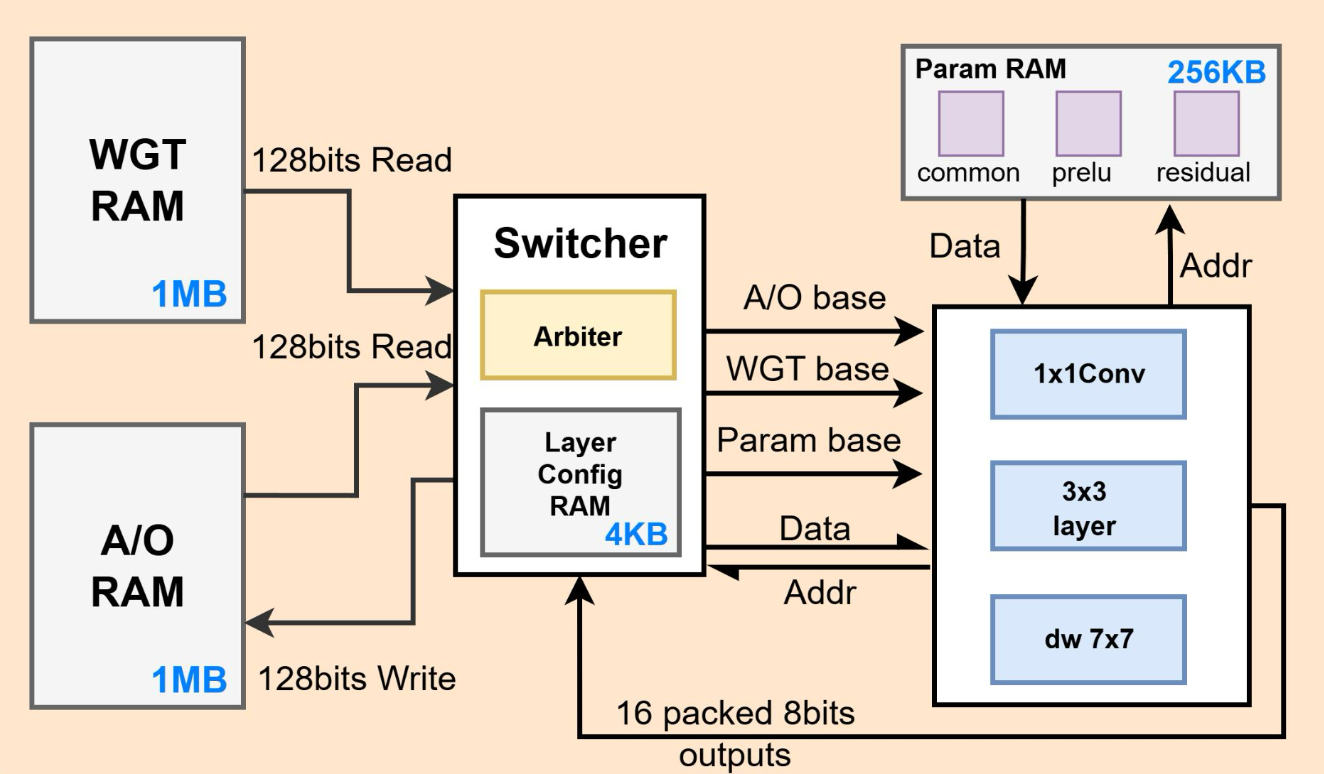
\includegraphics[width=0.9\textwidth]{Fig/peixing/Hardware_Architecture.png}
  \caption[NPU top-level architecture.]{NPU top level. The Switcher routes the active layer descriptor and data between the global memories (WGT RAM, A/O RAM, Param RAM, Layer Config RAM) and one of three operator engines: $1\times1$ Conv, $3\times3$ Layer, or dw $7\times7$.}
  \label{fig:npu_top}
\end{figure}

\paragraph{Global memories.}
Table~\ref{tab:npu_memory} lists the four shared memories. Sizes are the FPGA-side BRAM allocations; the ASIC track keeps the same depth but realises the largest memories with different physical resources, as described in Section~\ref{sec:hw:backend:asic}.

\begin{table}[H]
\centering
\caption{NPU Global Memory Hierarchy}
\label{tab:npu_memory}
\begin{tabular}{lll}
\toprule
\textbf{Memory} & \textbf{Size} & \textbf{Contents} \\
\midrule
WGT RAM         & 1\,MB         & Quantised INT8 weights for all 50 layers \\
A/O RAM         & 1\,MB         & Input activations and intermediate/final outputs \\
Param RAM       & 256\,KB       & Per-layer common params + PReLU $\alpha$ + residual offsets \\
Layer Config RAM& 4\,KB         & 64-bit layer descriptors driving the Switcher \\
\bottomrule
\end{tabular}
\end{table}

\paragraph{Switcher and execution flow.}
On each layer the Switcher reads the next 64-bit descriptor from the Layer Config RAM, decodes the operator type and the WGT / A/O / Param base addresses, and selects the matching operator engine. The PS-side host needs only to write the start address and assert a start signal: the Switcher walks through the 50-entry descriptor table and stops when the last layer completes, at which point the 128-d embedding has been written back into the A/O RAM ready for AXI readback.

\paragraph{Compute datapath summary.}
The three engines reuse a common Window Generator $\rightarrow$ array $\rightarrow$ Post-Process pipeline. The Window Generator slices A/O RAM into per-cycle patches; the array (sized to the operator) does the multiply--accumulate; the Post-Process unit applies bias addition, requantisation back to INT8, residual add, and PReLU before packing 16 outputs into a 128-bit write back into A/O RAM. Detailed datapaths for the $1\times1$ Conv and $3\times3$ Layer engines follow in Section~\ref{sec:hw:frontend:engines}; the design rationale (Why systolic array, why $14\times16$, quantisation scheme) is presented in Section~\ref{sec:hw:frontend:rationale}.
